\documentclass{standalone}
\usepackage{tikz}
\usetikzlibrary{angles, quotes}

\begin{document}


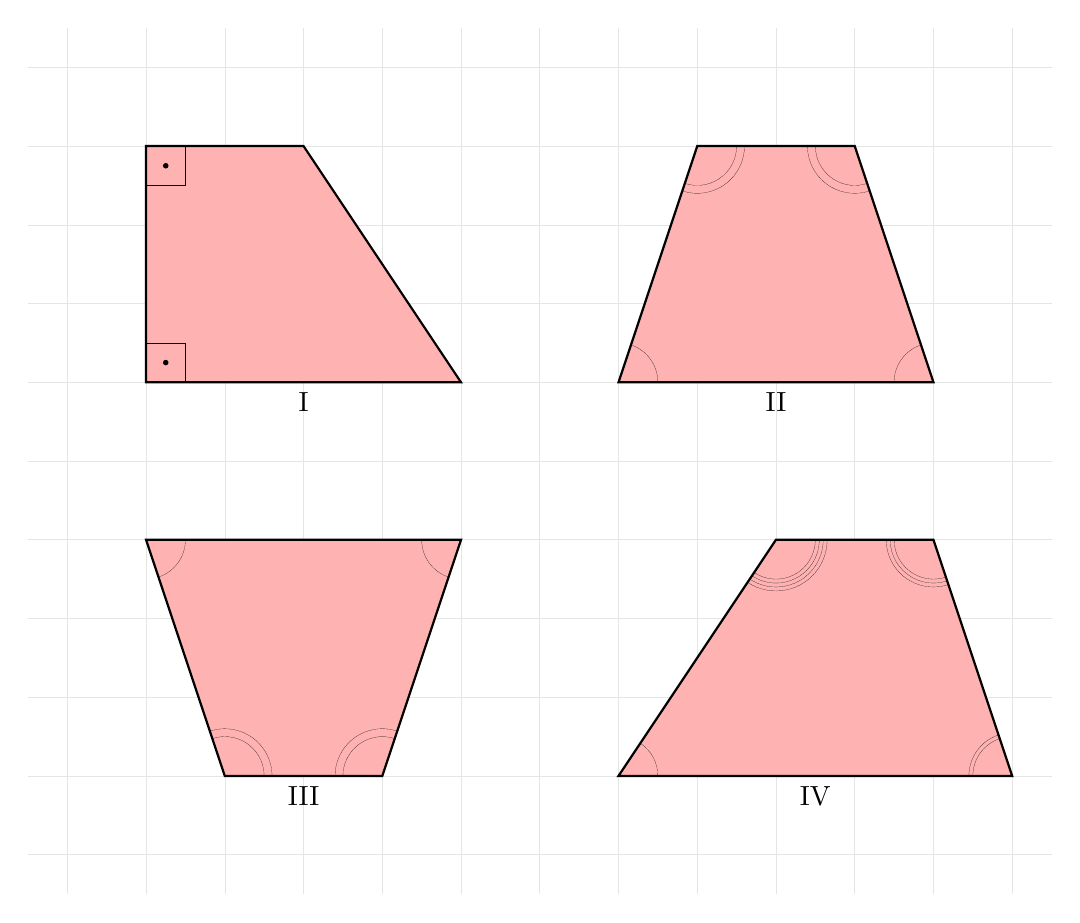
\begin{tikzpicture}
  \draw[help lines,black!10] (-6.5,-5.5) grid (6.5,5.5);
%  \draw[thick,->,red!20] (0,-5) -- (0,5) node[left]  {y};
%  \draw[thick,->,red!20] (-5,0) -- (5,0) node[below] {x};
%  \foreach \x in {-4,-3,-2,-1,1,2,3,4} \node[left,color=red!20] at (0,\x) {\x} node[below,color=red!20] at (\x%,0) {\x};
%  \node[below right,color=red!20] at (0,0) {0}; 





% Polígono A
\draw[thick,fill=red!30]     (-5,1) coordinate (A1)
      		 -- (-5,4) coordinate (A2)
      		 -- (-3,4) coordinate (A3) 
      		 -- (-1,1)  coordinate (A4) 
      		 -- cycle node[midway,below] {I};

% "A1"
\draw (A2) pic [line width=.05pt, draw, angle eccentricity=1.5, angle radius=5mm] {right angle=A4--A1--A2};
% "A2"
\draw (A3) pic [line width=.05pt, draw, angle eccentricity=1.5, angle radius=5mm] {right angle=A1--A2--A3};
% "A3"
%\draw (A4) pic [line width=.05pt, draw, angle eccentricity=1.5, angle radius=5mm] {angle=A2--A3--A4};
% "A4"
%\draw (A1) pic [line width=.05pt, draw, angle eccentricity=1.5, angle radius=5mm] {angle=A3--A4--A1} +(.25,.25) [fill] circle (.5pt);
\path (A2) +(.25,-.25) [fill] circle (1pt);
\path (A1) +(.25,.25) [fill] circle (1pt);



% Polígono B
\draw[thick,fill=red!30]     (4,4) coordinate (A1)
	         -- (5,1) coordinate (A2)
	         -- (1,1) coordinate (A3) node[midway,below] {II}
	         -- (2,4) coordinate (A4) 
	         -- cycle;

% "A4"
\draw (A1) pic [line width=.05pt, draw, angle eccentricity=1.5, angle radius=5mm] {angle=A3--A4--A1};
\draw (A1) pic [line width=.05pt, draw, angle eccentricity=1.5, angle radius=6mm] {angle=A3--A4--A1};
% "A1"
\draw (A2) pic [line width=.05pt, draw, angle eccentricity=1.5, angle radius=5mm] {angle=A4--A1--A2};
\draw (A2) pic [line width=.05pt, draw, angle eccentricity=1.5, angle radius=6mm] {angle=A4--A1--A2};
% "A2"
\draw (A3) pic [line width=.05pt, draw, angle eccentricity=1.5, angle radius=5mm] {angle=A1--A2--A3};
% "A3"
\draw (A4) pic [line width=.05pt, draw, angle eccentricity=1.5, angle radius=5mm] {angle=A2--A3--A4};



% Polígono A
\draw[thick,fill=red!30]     (-4,-4) coordinate (A1)
       		-- (-5,-1) coordinate (A2)
       		-- (-1,-1) coordinate (A3)
       		-- (-2,-4) coordinate (A4) 
       		-- 		   cycle node[midway,below] {III};

 
 % "A4"
 \draw (A1) pic [line width=.05pt, draw, angle eccentricity=1.5, angle radius=5mm] {angle=A3--A4--A1};
 \draw (A1) pic [line width=.05pt, draw, angle eccentricity=1.5, angle radius=6mm] {angle=A3--A4--A1};
 % "A1"
 \draw (A2) pic [line width=.05pt,  draw, angle eccentricity=1.5, angle radius=5mm] {angle=A4--A1--A2};
 \draw (A2) pic [line width=.05pt,  draw, angle eccentricity=1.5, angle radius=6mm] {angle=A4--A1--A2};
 % "A2"
 \draw (A3) pic [line width=.05pt, draw, angle eccentricity=1.5, angle radius=5mm] {angle=A1--A2--A3};
 % "A3"
 \draw (A4) pic [line width=.05pt, draw, angle eccentricity=1.5, angle radius=5mm] {angle=A2--A3--A4};




% Polígono A
\draw[thick,fill=red!30]     (6,-4) coordinate (A1)
	          -- (5,-1) coordinate (A2)
	          -- (3,-1) coordinate (A3)
	          -- (1,-4) coordinate (A4) 
	          -- cycle node[midway,below] {IV};

% "A4"
\draw (A1) pic [line width=.05pt,draw, angle eccentricity=1.5, angle radius=5mm] {angle=A1--A4--A3};
% "A1"
\draw (A2) pic [line width=.05pt, draw, angle eccentricity=1.5, angle radius=5mm] {angle=A2--A1--A4};
\draw (A2) pic [line width=.05pt, draw, angle eccentricity=1.5, angle radius=5.5mm] {angle=A2--A1--A4};
% "A2"
\draw (A3) pic [line width=.05pt,draw, angle eccentricity=1.5, angle radius=5mm] {angle=A3--A2--A1};
\draw (A3) pic [line width=.05pt,draw, angle eccentricity=1.5, angle radius=5.5mm] {angle=A3--A2--A1};
\draw (A3) pic [line width=.05pt,draw, angle eccentricity=1.5, angle radius=6mm] {angle=A3--A2--A1};
% "A3"
\draw (A4) pic [line width=.05pt,draw, angle eccentricity=1.5, angle radius=5mm] {angle=A4--A3--A2};
\draw (A4) pic [line width=.05pt,draw, angle eccentricity=1.5, angle radius=5.5mm] {angle=A4--A3--A2};
\draw (A4) pic [line width=.05pt,draw, angle eccentricity=1.5, angle radius=6mm] {angle=A4--A3--A2};
\draw (A4) pic [line width=.05pt,draw, angle eccentricity=1.5, angle radius=6.5mm] {angle=A4--A3--A2};

  

\end{tikzpicture}
	

 % \tikz
 %    \draw (0,0,0) coordinate (O)
 %      (1,0,0) coordinate (A) -- (O)
 %      (0,0,1) coordinate (B) -- (O)
 %      (0,1,0) coordinate (C) -- (O)
 %      pic [fill=gray,angle radius=4mm] {right angle = A--O--B}
 %      pic [draw,red,thick,angle eccentricity=.5,pic text=.]
 %        {right angle = A--O--C};




\end{document}
